\documentclass[a4paper,12pt]{article}
\usepackage[english]{babel}
\usepackage{graphicx}
\graphicspath{ {images/} }
\usepackage[font=it,labelfont=bf]{caption}
\usepackage{algorithm}
\usepackage{algpseudocode}
\usepackage{varwidth}
\usepackage{amsmath}
\usepackage{amsthm}
\usepackage{subcaption}
\usepackage{float}
\usepackage{titlesec}
\usepackage{cleveref}
\usepackage{cite}
\usepackage{url}
\usepackage{harvard}
\usepackage{thm-restate}
\usepackage[space]{grffile}

\citationmode{abbr}


\linespread{1.3}

\captionsetup[subfigure]{subrefformat=simple,labelformat=simple}
\renewcommand\thesubfigure{(\alph{subfigure})}

\setcounter{secnumdepth}{4}
\newcommand{\myparagraph}[1]{\paragraph*{#1}\mbox{}\\}

\newtheorem{theorem}{Theorem}[section]
\newtheorem{lemma}[theorem]{Lemma}
\newtheorem{defin}{Definition}
\newtheorem*{objective}{Objective}
\newtheorem*{rquestion}{Question}
\newtheorem{subobjective}{Sub-objective}
\newtheorem{subquestion}{Sub-Question}
\newcommand{\mydef}[3]{
\begin{defin}
\textsc{#1}

Given: #2

Question: #3
\end{defin}}

\newcommand{\bigO}[1]{$\mathcal{O}$($#1$)}
\newcommand{\bigOs}[1]{$\mathcal{O^*}$($#1$)}
\newcommand{\NP}{$\mathcal{NP}$}
\newcommand{\acco}[1]{\{ #1 \}}

\newcommand{\vecarr}[3]{\overset{#2}{\overrightarrow{#1}}}

%Door deze regel springt de eerste regel van
%elke alinea niet meer steeds een stukje in.
%\setlength{\parskip}{\baselineskip}
%Door deze regel wordt tussen de alinea's steeds
%een regel overgeslagen.

%\setlength{\columnseprule}{1pt}
%\def\columnseprulecolor{\color{blue}}

\newcommand{\algorithmicbreak}{\textbf{break}}
\newcommand{\Break}{\State \algorithmicbreak}



\begin{document}
\title{Simulation and Optimisation of Offshore Renewable Energy Arrays for Minimal Life-Cycle Costs}
\author{Robin Kuipers \\[1cm] Supervisors: \\ Kerem Akartunali \\ Euan Barlow\\[2cm] University of Strathclyde \\ Strathclyde Business School \\ {\small Glasgow, Scotland}}
\date{January, 2020}

\maketitle

\pagebreak

\begin{abstract}
This report aims to give a detailed overview of the research progress I made between March 2018 and September 2019, the first year of this PhD project into logistical decisions regarding offshore wind farms. It will explain the research subject, give an overview of the relevant literature I've read and the limitations of the current research. Furthermore, it will discuss the work I've done on a simulator, to be used for later research. Finally, the next steps and ultimate goals of this project are described. 
\end{abstract}

\pagebreak

\tableofcontents

\pagebreak

\section{Introduction} \label{s:intro}
%TODO: Add refs for `several years' and `30 years' claims
Over the past year, I have been researching logistics related to offshore windfarm projects; the installation, maintenance, and decommissioning of windfarms in various seas and oceans, primarily the North Sea. The installation and decommissioning projects can often take up to several years, and the lifespan of such farms is about 30 years, over which maintenance has to be done. For these projects, expensive vessels have to be used, the rent of which is often upwards of \pounds 100.000 per day \cite{barlow2014support}, hence a project with multiple vessels over many months can cost upwards of \pounds 100 million \cite{kaiser2010offshore}. Therefore, even small improvements to the schedules can save significant amounts of money.

Because of this, I expected a lot of research in this area had already been conducted, but this turned out to be less the case than I would have expected. Most research is fairly recent, and there are significant literature gaps. The primary obstacle in this logistics problem which separates it from more traditional logistics problems is the high degree of nondeterministic factors, mainly related to the weather conditions. These projects take place on open sea, where weather can often be rougher than on land. In addition, the high-tech vessels are performing operations on large industrial constructions, hence there is a limited range of allowed wind speeds and wave heights. Something else which can further limit possible schedules is the inflexibility involved in vessel rental, since vessels of the required calibre cannot be rented on short notice, and often need to be rented for at least some minimum amount of time \cite{kerkhove2017optimised}, so adaptive in-the-moment scheduling is impossible and we cannot simply wait for an expected period of good weather based on real-time data to rent the vessels; if we expected some period to have good weather but this turns out not to be the case, we will often have the vessels rented but unusable. This means the problem has a lot of nondeterministic factors which have a large impact; factors which any good solution approach will have to take into account. 

In this report I will talk about my progress and what I have learned over the past year. First, in \Cref{s:project}, I will explain the examined problem in more detail, and introduce the goals of this research project. After that, in \Cref{s:lit}, I will recount the reading I have done so far, which was the main focus of my work over the past year. This will include both research on this specific project, and research in the more general fields of (stochastic) scheduling and common methods such as optimisation and simulation. This will be the main focus of the report, as it was the main focus of my work. In addition to reading up on the state of the current research, I have also started building a Simulation tool for this problem, which I will discuss in \Cref{s:sim}. My other activities, such as some courses about research that I followed, are summarised in \Cref{s:otact}. Finally, I will summarise my current standing and plans for future work in \Cref{s:concl}. 

\pagebreak

\section{The project} \label{s:project}
In this section I will describe my research project in more detail, and discuss the questions I aim to answer by the end of it. This should provide sufficient context for the rest of the report. 

My project is about optimising all sorts of logistical decisions regarding offshore energy sites, primarily windfarms. This includes supply chains, routing, design of the windfarm, and scheduling of the operations to be done on the windfarm. The latter is where my primary focus lies, and what the majority of this report will be about. 

\subsection{Logistical decisions on offshore windfarms} \label{ss:logdec}
The type of offshore windfarm (OWF) this research project will focus on is described in \cite{barlow2018mixed}. A typical windfarm of this type will have two types of structures: Wind Turbine Generators (WTGs) and Offshore Substation Platforms (OSPs). The WTGs are the actual turbines generating energy, and the OSPs are hubs where the power generated in the WTGs is gathered and transformed before being transported to shore. Between these structures are many cables, connecting the WTGs to the OSPs, generally with a number of sets of WTGs connected serially. Then from each OSP there are specialized cables back to shore. A typical OWF currently in development might have upwards of 100 WTGs and 2 OSPs \cite{ruk2017}. 

The life-cycle of an OWF can be broken up into three phases: installation, maintenance and decommissioning. Installation and decommissioning are similar in structure; a fixed set of tasks needs to be completed in a cost-effective way. The primary difference is the reversed order of the tasks. For each of the structures there is a set of tasks that need to be completed in series for each individual structure, such as (for installation): preparing the sea surface, laying the foundation, installing the structure and laying the cables (each of these tasks may be split into more tasks such as loading, transport and installation) \cite{kerkhove2017optimised}. Within the group of tasks for a structure, most tasks will have to be performed in a specific order, while the tasks for separate structures can be completed in any order. This is essential for some of the more sophisticated objective functions used in the literature; if one OSP and a set of WTGs connected to it are active, they can start generating power while the rest of the wind farm is still under construction \cite{barlow2017using}. This is often a contractual requirement imposed by the government, and it would also mean the farm starts making money significantly earlier, and can therefore have significant impacts on desired schedules. This can lead to contractually or legally enforced deadlines for certain milestones, like 10\% or 50\% of the WTGs being operational.

The structure of maintenance projects is completely different. The set of tasks in not fixed, and ideally maintenance would only be performed right before an asset was about to fail. However, this is impossible to predict, and due to long lead up times of renting maintenance vessels waiting for an asset to fail will cause long periods of downtime. Scheduling maintenance has to be done significantly in advance. It is also costly, meaning maintenance trips which would have been unnecessary are undesirable as well. These two factors mean an efficient maintenance policy needs to find a balance between not spending too much on maintenance, and maintaining high uptime on the structures of the site (especially OSPs being offline can lead to massive losses in profit). 

%TODO: Possibly add something about subjectivity, and the goal not being finding a `perfect' schedule but a number of candidate schedules
The stochastic nature of the project also comes with various challenges. Naively one would perhaps go for the schedule with the lowest expected cost or the earlier expected end time. But the specific goal depends on the wishes of the executing company and project details. For example, a company may want at least 95\% certainty that the project is complete (or complete up to some milestone) by a given deadline, or some certainty that the costs do not exceed a given threshold. Therefore the probability distribution of the cost and duration of a resulting schedule are important to determining the value of that schedule. Additionally it is worth noting that while the end time of a schedule and the cost are strongly related, there are scenarios in which it is more profitable to halt the operations for a number of months, especially the winter months where there will be more days with weather too extreme to perform operations in. While this break would obviously postpone the total completion of the schedule, not having to pay rent for vessels over these months in which they cannot perform optimally might lead to a higher net profit over all, especially if a part of the windfarm is already operational and generating energy over these months. In this way, schedules need to be determined on various levels; there are day-to-day decisions, and much larger decisions regarding operational periods. 

%TODO: For the cites, look at sources and where they got it from; citing directly leads me to more (varied) sources

\subsection{This research project} \label{ss:objs}
The primary goal of this project is to look at the entire life-cycle of OWFs, and how decisions at different points in this life-cycle impact the situation at other points in time. Specifically I aim to use both optimisation and simulation to provide insight into logistical decisions, primarily scheduling, but potentially also layout of the site and the routing on it. The latter two are very challenging subjects on their own, and I will likely only run simplistic experiments with them, to see whether looking at a full life-cycle gives any insights on its own. Therefore the primary focus will lie on scheduling, specifically scheduling that considers the entire life-cycle. 

Over the past year, I have spent most of my time reading up on the subject, both the methods and the challenges of offshore projects. This literature is summed up in \Cref{s:lit}. Additionally I have been laying the groundwork for a simulator which I am planning to turn into a tool for support on the logistical decisions described previously. Details on this tool are given in \Cref{s:sim}.

\bigskip

The primary research question is:

\begin{restatable}{rquestion}{rquest}
Can considering the entirety of the life-cycle of an Offshore Wind Farm, and how each of the phases interact, improve logistical decision making on these projects?
\label{rquest}
\end{restatable}

The primary motivation for this objective is that in the literature the three phases of the life-cycle are each treated separately, while they might heavily influence each other. There is a large amount of research done on the maintenance projects, and quite a bit on installation projects as well, while decommissioning projects are less well researched. However no research was found considering all three phases simultaneously. Treating these phases as separate makes them more manageable, but some insight about how they influence each other is also valuable. There are two primary ways in which these phases interact; some partially take place at the same time and share resources, and any phase affect any phase after it. 

For the first type of interaction it is important to consider that the maintenance phase overlaps with both other phases for some amount of time. Once the first set of wind turbines has been fully installed they start producing energy and might require maintenance, while the rest of the turbines are still being installed. It may be beneficial to use the same vessels to install the remaining wind turbines and perform maintenance, or have separate vessels that still use the same ports and have to consider the routing of the installation vessels. The same thing happens at the end of the life cycle; when decommission starts specific wind turbines are decommissioned while others continue to produce energy. 

%TODO: Cite someone regarding the possible explanation for low decomisison research
The second type of interaction has to do with any event in the life-cycle of a wind turbine (or the entire farm) affecting all events that come after it, regardless of which phase these events are part of. The order in which the turbines are installed determines their age, and affects their expected failure rate when maintenance starts on them. In a more extensive way, any failures and repairs during the maintenance phase influence which wind turbines are most likely to fail again, and therefore which are most efficient to decommission first. With that in mind it is clear that decommission is the phase which relies most heavily on what happens before it, which may be one of the reasons why it has been studied less than the other two phases. This type of interaction means simulating the early stages of the life-cycle of the windfarm might lead to more accurate and realistic knowledge to base decisions in the later stages of the life-cycle on. For example, basing the order in which turbines are decommissioned on their actual history of failures and reparations is expected to lead to better result than a predetermined arbitrary order. 

This interaction works in the other direction as well. Instead of the history of the windfarm influencing decisions near the end of the life-cycle, the future of the windfarm can also influence early decisions. For example, if we compare two installation schedules and base our choice solely on a measurement done during the installation phase (such as the date the installation finishes, or the cost at time of finishing) this could potentially lead to another option than if we look at the entire life-cycle. Non-operational periods are times of the year (usually winter months) in which no installation operations are performed on the site due to the severe weather conditions. Using periods like this leads to larger age differences between turbines, which could influence the maintenance and decommission phases. This effect cannot be fully measured unless the entire life-cycle is considered, and knowing the effect could influence decisions regarding the non-operational periods. 

Through these interactions we state three sub-questions for the above research question:

\begin{restatable}{subquestion}{sq1}
\label{sq1}
Can considering how phases in the life-cycle of a windfarm overlap and share resources improve logistical decision making on these projects?
\end{restatable}

\begin{restatable}{subquestion}{sq2}
\label{sq2}
Can simulating the entire life-cycle of a windfarm provide useful data to base logistical decisions on in the later phases of these projects?
\end{restatable}

\begin{restatable}{subquestion}{sq3}
\label{sq3}
Can considering the long-term effects of logistical decisions early on in the life-cycle of a windfarm improve these decisions? 
\end{restatable}

While the latter two questions seem similar, they approach the same phenomenon from different perspectives. This will likely lead to different techniques and models being used to answer them. 

\pagebreak

\section{Literature} \label{s:lit}
In this section I will give an overview of the literature I have read to-date for this research. I will discuss some actual attempts to produce a schedule for the installation problem in \Cref{sss:sched}, and research on the maintenance of the site will be shown in \Cref{sss:maint}. Other research related to offshore projects is shown in \Cref{sss:offsh}. Some other studies to do with uncertain scheduling will be highlighted in \Cref{sss:stoch}.  Afterwards in \Cref{ss:meth} the theory and development of common methods for these problems will be discussed.

\subsection{Research overview} \label{ss:rese}

\subsubsection{Scheduling the installation} \label{sss:sched}
Here I will take an in-depth look into two papers that use comparable methods to look at the issue of producing an efficient schedule, and discuss their strenghts, weaknesses, and difference.

\bigskip

In \cite{barlow2018mixed} a mixed-method approach is used. They identify the strengths and weaknesses of both simulation and optimisation, and aim to use the methods together in a way that utilises the strength of each. First a simulation is used to determine some amount of delay before starting the project, as this can have sizeable impact on the total duration of the project. Then, a mathematical programming model is used to construct a schedule from this starting point. The output of that optimisation model is then used in the simulation to give a view of the overall costs under uncertain circumstances. 

For the simulation a synthetic weather time-series model is used. This weather model is described in full in \cite{dinwoodie2014operational} , and uses a correlated auto-regression model which identifies underlying trends in the data and aims to predict future behaviour over time. This seems to be a fitting and sophisticated model. However, in the optimisation model a more simplistic model is used. Tasks are given a minimal duration $d_{i, min}$ and a maximum increase $d_{i, inc}$ of that duration. The realised duration is given by $d_{i,  min} + z_i d_{i, inc}$ for some $0 \leq z_i \leq 1$. The programming model has two levels; the outer model maximises $\sum_i z_i \leq \Gamma$ for some given limit $\Gamma$. The inner model then uses the fixed values $z_i$ to set the start times of each task in accordance with their deadlines and precedence relations. 

In effect, a $\Gamma$ is chosen to represent a certain percentage of tasks taking their maximum duration. For example, if there are 200 tasks and 10\% of them can take the maximum duration, $\Gamma$ is set to 20, and this can either result in 20 tasks taking their maximum duration with all other tasks being completed in the minimum duration, or every task taking 10\% of its maximum extra time ($d_{i, inc}$). 

\bigskip

I have a number of criticisms about this research, which I will now discuss.

The way delay is modelled in the optimisation model considers delays independent, while in practice there are clear patterns. Often multiple vessels are used, meaning multiple tasks are scheduled for the same time. If one of the tasks is delayed due to the weather, any other tasks scheduled for that time will have to be done under the same weather conditions and are therefore more likely to be delayed. The same holds for two tasks done concecutively by the same vessel, as the weather conditions will be similar for these tasks. 
Another criticism of the way delays are modelled tasks have a maximum amount of time they could be delayed, but other papers in this field (including the one discussed in the latter half of this section) mention than many tasks cannot be performed at all under certain weather conditions. This is structurally different behaviour from a task simply taking longer, as it may delay any of that type of task for hours or even days. This behaviour is still included in the simulation, so it is tested for when evalutating the quality of a schedule. However it seems the schedules could be improved if this behaviour was considered in the optimisation model as well. 

An additional criticism to make this research more applicable is the objective function used in optimisation. The makespan of the longest path of the schedule is minimised, but a company doing the installation will often be more interested in the total cost of a schedule. This is clearly very related to the makespan, but can differ if certain vessels are used for longer than others, and when parts of the OWF can become active (and generate profit) earlier. Early completion of sections of the windfarm are currently treated as certain milestones to reach, but when using the monetary value of the project in the objective function the actual financial benefits of early completion take effect. The common practice of discounting the cost and value future spending and profit could also be incorporated in this to more accurately represent the interests of the company. It seems like more research into this could therefore be beneficial. 

Finally the strengths of the simulation could be utilized more. In the research presented, a start date is determined at the start and this is then used in the optimisation and for the rest of the research. However in determining a start date a very rudimentary schedule is used. Optimal schedules starting in each month could be explored more, as well as pausing the operations after they started. For example, if the winter months turn out to be very difficult and slow to work in, the project could be paused over several months, over which no rent for the vessel would have to be payed. This would seem to be particularly effective if a subset of the WTGs could be operational before pausing, as they would generate energy (and revenue) during winter. These periods of time are called non-operational periods, and are sometimes used in large projects such as these.  

\bigskip

A different model is designed in \cite{kerkhove2017optimised}. It uses similar methods as used in \cite{barlow2018mixed}, namely a mixed-method of optimisation and simulation, but in a significantly different way. The research incorporates certain industry restrictions to do with vessel renting; it keeps track of which dates vessels are commissioned and decommissioned, incorporates a price for both, and has restrictions on minimal renting and downtime periods. These logically make sense, as the vessels likely have costs to travel between the storage and used port, and the rental company will usually not be able to find other uses for a vessel if it has a sort down time. 

A thing of note about this research is the advanced weather simulation model used for the simulation. It uses a combination of transition probability matrices and a Weibull distribution to generate wind speeds and wave heights that are both sufficiently correlated to each other and themselves. The data this is based on was divided by month of the year, so the model takes time of year into account. Given the degree to which this type of project depends on the weather conditions, a realistic and sophisticated model like this is very beneficial for the applicability of the model. 

Related to the financial focus of this research, the variables being decided on are the gate times of the tasks, instead of the start times as previously. The gate time refers to the time from which resources for a certain task should be made available. These times should be determined in advance, as there are generally long lead times associated with renting the vessels (hence they do not lend themselves much for dynamic scheduling). This allows for the optimisation to directly influence when the money is spent, which is a major focus of this research. The objective function is also different to accommodate this, it maximises net present value of the complete project. This takes into account discount rates both on expenses and project value, which are emphasised in the literature. These discount rates are higher than commonly used in research such as this, with the rationale that the main reason to include discount rates is the inherent uncertainty of the future, and projects of this nature have an exceptionally high degree of uncertainty.

Before determining the gate times, the project is divided into time periods. Any size of time period could be used, but in this particular research they choose to use months. Then for each month and each type of task a decision is made whether that type of task can be performed in that month. Each of these decisions is called a chromosome, and a collection of them (for each combination of months and tasks) is called a gene. From the gene a set of gate times is generated through a simple algorithm, and this schedule of gate times is tested in simulation. From there, the gene is modified and tested again, until some end condition is reached. 

Three different methods are compared for this process. Two of them are forms of local search; a simulated annealing algorithm is used to find optimal genes. The difference is the type of gene that is used; one distinguishes between different years, the other does not. That is to say, one treats July in year 1 and July in year 2 as different months with different restrictions on tasks while the other does not. The other method is a heuristic instead of local search. Each task is set to have equal weather requirements, meaning that a month either allows for all tasks, or allows for none of them. The other big simplification made in the heuristic is that only a single non-operational period is chosen, which repeats every year. These two strong restrictions mean there are only two decisions to be made; the month in which the non-operational period starts, and the month in which it ends. This reduces the solution space to $12^2 = 144$ different possible genes, all of which is tested and the optimal one is selected. In the experiments performed, this dedicated heuristic search outperformed both methods of local search . 

\bigskip

As with the previous paper, I will now discuss my criticisms of this research. 

The three methods compared above are seen as separate, but they can potentially be combined to improve results. The dedicated search heuristic performed best, but the gene it comes up with will always be simplified. If it is used as a base, after which its best performing results are used as starting solutions for either of the local search methods, it could lead to better results as the solution space that is explored is expanded around areas that have been shown to perform well. 

I also think the way genes are used could be improved. They are fairly high level, as they determine which (category of) tasks can be performed in which month, but determining the schedule on a more detailed timescale can likely lead to much better results. In the paper a conversion algorithm is used to generate gate times for each task based on any given chromosome, but it is very simplistic. It is assumed none of the tasks have a weather delay, and every task is placed immediately after all preceding tasks should be completed. A simulation is used to test this schedule, and if any task executions violate the given chromosome the gate time of that task is shifted forward to the next eligible period. However this is done using a single simulation, which does not say much about the expected outcome. This seems like a very simplistic method to use (as the genes operate on a much larger timescale than the gate times) and leads me to think improvement might be very beneficial. How exactly this is to be done can be discussed, but using more than a single simulation will generally be a good start. Potentially this method can be used to determine non-operational periods, but a more complex optimisation for the day-to-day schedule could be used after it, such as the one used in the previously discussed paper. 

A final big limitation of this research has to do with one of the cashflows being ignored. While the monetary value of the project is presented as the main focus, there is no mention of any positive cashflow starting when the project is partly done, nor are there any deadlines for milestones mentioned (such as when the first 10\% or 50\% of the WTGs are operational). Therefore the only positive value considered in the objective is the fixed value of the project upon completion, subject to discount rates. For research so focused on the financial perspective, not incorporating the possibility of early positive cashflows seems like a big gap, and a possible improvement for future research.

\subsubsection{Maintenance of the site} \label{sss:maint}

Compared to the topic of installation, there is a large body of research done in the area of operation and maintenance (O\&M) of offshore wind farms. This research looks at various aspects and timescales relevant to the OWFs. In \cite{shafiee2015maintenance} the research and topics are divided into three timescales (echelons):

\begin{enumerate}
\item Strategic: Long term, over the lifespan of an OWF
\item Tactical: Medium term, between 1 and 5 years
\item Operational: Short term, day to day
\end{enumerate}

Within each of these echelons, various areas of research are identified. Strategic decisions are found to have the biggest impact on the costs of operations, which makes sense as they affect the largest amount of time. However each of these echelons include important decisions that will have to be made for the maintenance of the sites. 

One aspect to consider is fleet size. In \cite{staalhane2019optimizing} a two-stage stochastic programming model is used to first determine which vessels to charter, and then how to use the cartered vessels. In their computational study this approach is compared to several life-cycle cost estimating simulation models from the literature, and it is found to give reasonable estimates on the resulting costs. Additionally it is shown to require relatively low computational power, and can therefore be used to support maintenance decisions made. 

With the large amount of research done, and the variety of subjects within this field, I have yet to read much more about the current state of most subjects. This will be my immediate focus from here on, as described in more detail in \Cref{s:concl}.

\subsubsection{Related research regarding offshore projects} \label{sss:offsh}
While there is not much research relating specifically to decommission projects, there is some. Especially recently there has been new research such as \cite{irawan2019optimisation}. In it the researchers use an Integer Linear Programming method to find schedules for decommission projects with minimum costs. The method is shown to be efficient and seems to yield good results. As expected, this model is fairly similar to the ones used for installation projects. 

\bigskip

A group of researchers at my department, whose research \cite{barlow2018mixed} I have already described in \Cref{sss:sched}, have developed a simulation tool with which various logistical decisions for the installation of an OWF have been explored. In \cite{barlow2014support} the number of installation vessels and supply barges is experimented with, as well as their relative release dates. These simulations consider only the installation of OSPs and not WTGs. There are several measures considered for the quality of a setup such as the total cost of the project and the completion dates of the first and last OSPs, as well as the uncertainty of those measures (shown through the median and 90\% confidence interval for these measures, resulting from 100 simulations). 

In \cite{barlow2014assessment} the same tool is used to compare several types of installation vessels. Simulations are run with vessels varying in four measures; number of WTGs it is able to carry at once, transition speed, maximum wave height for transitioning and maximum wave height during jacking operations. The values tested range from those corresponding to current vessels to those corresponding to expected vessels available in the near future. The transitioning speed is the only measure which seems to yield continuing improvement; the other three measures have clear diminishing returns and improvement beyond vessels currently available is unlikely to be worth it (given that newer vessels will have a higher cost). A criticism I have of this research is that all measures are tested in isolation, while three of the four measures are directly related the number or length of transits between the port and the OWF site. It is plain to see that the average transitioning speed matters less when the capacity is high enough to limit the number of transitions. This is not mentioned in the paper.

In \cite{barlow2017using}, the final paper (so far) on this tool, the researchers go a bit more in depth on the tool and simulation as a method for supporting decisions in these projects. They talk about how the model was constructed and how after each round of improvements the model was validated with industry partners to ensure it accurately models reality. Some experiments are also discussed, the first being a simple simulation of the installation of a fictional OWF over 1000 weather series. The costs and duration of each segment of operations are analysed, and it is shown to be desirable to reduce any uncertainty as distribution of costs has a long tail. The standard deviation is \pounds 11.80M (approximately 5\% of the \pounds 233.89M median cost) so reducing uncertainty could potentially lead to saving significant amounts of money. Then experiments with different number of supply barges are performed for the WTG jacket phase of the installation. A scenario is set up where these operations start a full year after the preceding phase of laying the foundations to ensure no delay is caused by that. Two sets of experiments are done, one with a single installation vessel and one with two installations vessels. For both scenarios similar patterns are found in the result; for the costs, there is an optimal minimum and increasing the number of supply barges from there slowly increases cost. The duration of the installation tends to only decrease very slowly from that optimal minimum as well. The statistical significance of their results are also tested, and some differences are found not to be statistically relevant. Finally, the impact of the relative starting dates of piling the foundations and starting jacket operations are explored. The start of laying the foundations is fixed at April 1st to optimally make use of the summer weather conditions. If the jacket operations would start at the same moment, there would be a lot of waiting and delays since the foundations for a specific WTG need to be completed before the jacking operations can begin. This increases costs, so delaying the start of these latter operations is beneficial. A good amount of delay found is about 90 days, as waiting longer means more severe winter weather conditions. However, if it is possible to wait out the winter and delay operations about 420 days the total cost can be minimised as waiting this long means there are no delays due to waiting for the foundations, and making optimal use of summer weather conditions. The downside of this is a significant increase in makespan of the entire project. The OWF developer will have to decide between these options. For a different OWF the actual values will obviously differ, but similar patterns could be found. All in all, this tool is shown to be powerful and useful for logistical decisions related to the installation projects. 

\bigskip

%TODO: Check these texts and references
In a very recent work \cite{leontaris2019decision}, researchers have looked into reducing the risk of supply disruptions. Due to the absence of sufficient historical data, they use expert judgement to analyse the risk of supply disruptions, using different weights to combine judgements from various experts. It was found that the combined judgement lead to a better outcome than any individual judgement. In general it was found that not taking the estimations of supply disruptions into account could lead to significant overruns in both schedule and budget. 

The same authors have written about whether dependencies between task duration \cite{leontaris2018probabilistic} should be considered. They use a non-parametric Bayesian Network to model dependant delays in task duration, so that if a vessel has a delay on a certain task, the task it performs afterwards has a higher chance to be delayed as well. So far they have only tested this technique with the main tasks for installation, but this technique could be used throughout all operations. The initial results are promising, and ought to be considered in the design of my own models. 

In another paper \cite{leontaris2016probabilistic} the same authors attempt to generate synthethic weather series, where the different metrics (wave height, wind speed, and potentially more like wave period and wind direction) are dependent on each other. For this they use copulas, which join multivariate distribution functions. They test their method with a project for laying the cables of an OWF. Their initial results show that this method could provide more insights into the realistic durations of offshore projects. 

\bigskip

The problem of crew scheduling is discussed in detail in \cite{leggate2010crew}. In that, the problem of assigning specific crew members to specific tasks over long periods of time is considered. Each crew member has a number of contractual requirements, both on a small and a large scale. Any shift has a a maximum length, and if this crew member has to work outside that maximum length they get payed more. Additionally there is a maximum amount of time a crew member can be offshore. This is usually cut up in blocks of four or five weeks, as these contracts are standardised. There are also restrictions on the nationalities of the crew members. Ships with certain flags cannot employ certain nationalities, and the researchers state that certain combinations nationalities do not work well. All this leads to a rather complex problem, which is outside the scope of my research. It is too detailed for me to fully incorporate in my research, which focuses on a larger scale and decisions that effect the entire life-cycle. On top of that, as stated in this research these decisions regarding specific crew members generally lie with the company renting out the vessel and not the company renting it, while my research sees vessels as a resource to rent rather than own. However, there are still valuable insights in this research. For example it shows there will be contractual obligations to go back to the shore at a regular interval to ensure the crew does not spend too much time offshore. 

\bigskip

Another logistical decision topic related to the offshore windfarm sites is deciding their layout. This is discussed in various papers, such as \cite{mosetti1994optimization,kusiak2010design,saavedra2011seeding,perez2013offshore,hou2017combined}. There has been a significant amount of research in this direction, though most of this research focuses on windfarm on land, instead of offshore. The latter two papers \cite{perez2013offshore,hou2017combined} consider offshore windfarms, as this topic has gained more interest in recent years. While there is a large body of research, there are still many unanswered questions when one wants to determine how to get the most energy production from a site. One important question is the wake model to use, where wake is the decrease in energy output of a turbine based on the position of surrounding turbines. This is clearly a core part of determining where to place the turbines, and most wake models still have considerable uncertainty. A variety of methods to optimise turbine placement are used, where local search and genetic algorithms seem to be the most prevalent. While I am currently not planning to do significant research into the optimal methods to determine turbine placement, aspects of this research field are still very relevant as the wake influences the energy output of the site. Additionally the placement of the turbines can affect their failure rate and is therefore important when planning maintenance of the site. Therefore results found in the research of OWF layout will have to be incorporated in accurate models of those sites, and future research can potentially be done in this direction.

\subsubsection{More general work on stochastic scheduling} \label{sss:stoch}
%TODO: It's weird that I mention Robust Opt will be discussed in 3.2 and then the rest of this section is about robust as well. Fix? Restructure?
A comprehensive overview of various approaches to scheduling within an uncertain environment is given in \cite{herroelen2005project}. While the survey is relatively old, it provides a valuable categorisation of approaches used to handle uncertainty within scheduling problems. It discusses reactive scheduling, where the baseline schedule is made based on the assumption that all uncertain parameters will take their expected value, and any variation is handled at the moment it occurs. Stochastic project scheduling and fuzzy project scheduling are also discussed, as two different ways to handle uncertainty in project scheduling. Both share a weakness in that they do not produce reliable baseline schedules. For projects on OWFs this weakness is important, as contractors and companies renting out vessels have significant lead times and in-the-moment scheduling is infeasible in this situation. It is therefore crucial to have a baseline schedule which roughly corresponds to how the actual operations will turn out. This is what the last approach discussed in this survey provides; robust scheduling should lead to schedules that do not get disrupted easily. This method is discussed in more detail in \Cref{ss:meth}, as it is what I am planning to use for this research. Additionally the concept of sensitivity analysis is discussed, as giving related parties insight into the vulnerable parts of the schedule can often be beneficial. This is one of the goals of the tool discussed in \Cref{s:sim}. 

At the time of the above study not a lot of research had been done into robust scheduling. A work that had been published and is mentioned in the study is \cite{sevaux2002genetic}. It is one of the few works I was able to find which attempted to solve a robust scheduling problem using genetic algorithms. Their initial results seemed promising, but their industry partner stopped the collaboration before practical results were found. Since the initial results seemed promising and no reason was found that indicates genetic algorithms are not fit to be used for scheduling problems, this is one of the methods considered for my research, as discussed later in \Cref{ss:meth}.

\bigskip

A more recent overview of the state of robust optimisation is given in \cite{gabrel2014recent}. This study looks at 130 papers, 45 PhD dissertations, and selected other works published between 2007 and 2013 which discussed robust optimisation. The sheer amount of research done reflects the strength of this method. Both the theory and applications of robust optimisation are discussed, and some time is spend discussing its application for scheduling problems. 

%TODO: refine ?
In \cite{burke2010multi} a robust optimisation approach is applied to a multi-objective airline scheduling problem, the nature of which has certain similarities to offshore scheduling problems. Their approach, which used both iterative improvement and large-scale simulation, was tested in practice and yielded valuable results, signifying that a similar approach might yield good results for my research as well. 
Another study looking into robust scheduling is \cite{goren2008robustness}. It considers a single-machine scheduling problem where the machine randomly breaks down. A single-machine scheduling problem is comparable to a project at an OWF with a single vessel. The vessel temporarily having to wait out weather conditions would then relate to the machine breaking down. For this reason the findings in this study may be roughly applicable in offshore scheduling problems. However one key observation is that single machine scheduling problems often behave different from multi-machine scheduling problems, and most projects on OWFs will employ multiple vessels. 

As for research about the theory of robust optimisation, \cite{iancu2013pareto} introduces the concept of Pareto efficiency, which comes from economics and multi-objective optimisation. For a multi-objective problem a solution is Pareto efficient (also called Pareto optimal) if any change that gives a better value in one objective function will lead to a worse value in at least one other objective function. For such problems, any desirable solution will be Pareto optimal, and all Pareto optimal solutions together form the Pareto barrier. In \cite{iancu2013pareto} the writers state that within robust optimisation problems there will be a set of solutions which perform optimally within all tested worst-case scenarios, the so called Robustly Optimal (RO) solutions. They then identify some of these RO solutions to be Pareto Robustly Optimal (PRO), which means no other RO solution performs better than the PRO solutions across all possible scenarios. Effectively, they say that RO is not a strong enough requirement for solutions, as in reality the worst-case scenario will not often happen, and a solution being RO says nothing about how that solution will perform in a scenario which is not the worst-case. They then provide a method to generate a PRO solution from any RO solution in a time complexity not greater than the time complexity of the original problem, thereby not significantly increasing the time complexity to finding the desired solution. This paper is a couple of years old now, and their concept of Pareto Robustly Optimal solutions seems to have been used in various research papers since then. 

%TODO: CONTINUE here

\subsection{Research Methods} \label{ss:meth}
In the above literature, two main types of methods are used for this problem; optimisation and simulation. Often both are used together, either by tackling one part of the problem with simulation and another with optimisation (as in \cite{barlow2018mixed}), or by creating schedules with an optimisation model, which are then evaluated using simulation (as in \cite{kerkhove2017optimised}). In this section the methods will be discussed in more detail, separate from the research they were used in. Other possible methods for problems of the kind we are looking at will also be discussed. 

\bigskip

\subsubsection{Simulation} \label{sss:sim}
%TODO: 2nd line `accurate' said to be unclear and can a simulation be accurate
Simulation, especially Discrete Event Simulation, is a very broadly used method in computational analysis \cite{law2000simulation,robinson2010conceptual}. It is often used to evaluate the strength of a proposed layout or schedule under uncertain circumstances. If enough simulations are run, an accurate view of the realistic duration of a schedule can be gained. This does not only mean expected (average) duration, but also for example a confidence interval for the costs of the project or the probability a certain task will be completed before a set time. However, simulation for these offshore projects has two important bottlenecks; the information gained through simulation can only be as precise as the weather model used for it, and running enough simulations to get an accurate result can take considerable time. 

\bigskip

If the weather data is limited in precision or amount of data available, the applicability of the simulation results in turn will also be limited. A simulation as detailed as we would like for this type of project would have timesteps in the range of 15 minutes to an hour. A lot of weather data has much larger timesteps, often of several hours. There are methods to interpolate between weather data points, but this tends to not be very precise as there are a lot of factors to take into account. The most important measures of the weather are wind speed and wave height, as by these measures the usability of the vessels can be determined. In order for this data to be realistic, the two measures have to be correlated, as well as have autocorrelation over time. Having those values be realistically interpolated between two measured points is a difficult task, and something we will have to figure out a way to realistically handle for future research.

The amount of data available is also a common problem. A major reason for this is the natural change of weather depending on the time of year. Generally, a year would be split up in sections, for example the four seasons or the twelve months. Intuitively this makes a lot of sense; if we want to model the weather in January data from July is irrelevant for this. But the consequence is the sheer amount of time it takes to collect accurate data for each time period; if we want 300 days of data for the month of April, we need data collected over the span of 10 years. In addition, the conditions of the location the data is gathered from have to be similar to the location of the OWF. An important parameter for this is the distance to the shore, but there are more factors which play a part. 

A method to handle these drawbacks of the weather data is to not use raw data, but analyse the periodic characteristics of the change of both wind and wave states. Using these characteristics, one can generate weather data by drawing a random real data point within the desired time period, and extrapolating the data from there using the found characteristics. This is used frequently in the literature, and has been shown to have a good potential for stochastic simulations. 

Another method we are considering to explore relates more to robust optimisation. It might not be necessary to have a large number of simulations for all possible weather conditions. If, for each time period, we create a range of possible wind and wave states (including the extreme cases from the data) and run simulations for a set of (realistic) combinations of them we could aim to make a robust schedule that performs well within even the most extreme weather scenarios without having too many simulations to run. The drawback of this robust approach is a schedule that performs well in 99\% of weather cases might be discarded for the most extreme 1\% of cases. This can however be reduced by carefully selecting the data to use for the simulations, or allowing a certain number of bad scenarios (especially if the weather causing it is very rare). We might explore this more in future research. 

%TODO: Citations?

\bigskip

%TODO: Redo a lot of this cause it's repetative and unstructured
The other bottleneck, that of the considerable time it will take to run enough simulations, is something that will need to be taken into consideration for any research project using simulation. There are several methods to reduce the time used if necessary. A rigorous and effective step is increasing the size of a timestep. This reduces accuracy, but does significantly reduce calculation time as well. Another is to carefully select input so less simulations need to be run for precision, as was discussed above. Using a robust approach could potentially reduce the number of required simulations, as the robust inputs are constructed to explore important situations, instead of random inputs which require a lot of simulations to construct an accurate average. 

There are many other possible methods to reduce number of simulations required, and which to apply depends on the specific research project and goals, and how much speed is needed. This is something we are aware of for when experiments will be done in the future. 

\subsubsection{Optimisation} \label{ss:opt}
Optimisation, in particular through (mixed-)integer programming, is an essential tool in problems like this, and is used extensively in the literature \cite{nemhauser1999integer,lee2011mixed}. Linear programming and integer programming is preferred as mixed-integer programming is computationally much more complex to solve, therefore mixed-integer models are restricted in size in order to be solved in feasible time. However, both methods are used in the literature.

Even linear and integer programming models computationally complex to solve, hence many methods are used to reduce to complexity of the models. There are standard techniques like Lagrangian relaxation \cite{fisher1981lagrangian} and column generation \cite{barnhart1998branch}, but there are more specific methods used as well. The primary way this is done is by limiting the scope of individual optimisation problems (not necessarily the research), by splitting up the research and using multi-level optimisation models, or using simulation for certain parts of it. 

Another method has been discussed before already; robust optimisation. As with simulation, this reduces the number of considered inputs (primarily weather states, but also task duration which is sometimes stochastic) by only considering certain constructed uncertainty sets. This strongly reduces the number of situations considered in the optimisation. 

\bigskip

There are alternatives to computational programming. The most prominent are heuristic methods, such as local search. Heuristics are powerful when dealing with large problems like this, as finding an exact global optimum will usually take an infeasibly long time. A benefit of local search is that reasonably good results can often be found fairly quick, but this is connected to the main drawback of local search; it can often be difficult to get out of local optima. However, there is a lot of literature on local search and other heuristics and many variants designed to reduce its drawbacks. 

Alternatively, evolutionary algorithms have been used for deterministic scheduling problems such as machine learning \cite{dorndorf1995evolution}. A good explanation of this technique for scheduling is given in \cite{cotta2007memetic}. While this technique seems to be fairly common in deterministic scheduling, not much research could be found in an uncertain setting. The exception is \cite{sevaux2002genetic} as discussed in \Cref{sss:stoch}. This research, although seemingly brief, gives quality results. Since there is no clear reason why evolutionary algorithms couldn't work well within an uncertain setting, this is a potential method to explore in the future. 

\subsubsection{Combining Simulation and Optimisation} \label{ss:simopt}
When optimisation is to be performed within nondeterministic environments, it is often combined with simulation, such as in \cite{de2003integrating} and \cite{bard2015integrating}. A primary reason for this, and why I plan on using this too, is that simulation is a very effective way to analyse large-scale schedules subject to uncertain conditions. The optimisation and simulation model can be integrated by using the simulation to evaluate a schedule proposed by the optimisation model. This can often give more accurate results than using a simplistic objective function. The simulation model can then return an appropriate metric regarding the quality of the schedule, such as makespan or total cost, and the optimisation model can aim to improve from there. In theory this integration can even be extended; the simulation model can determine metrics relating to specific subsets of tasks, and potentially the optimisation model can use this extensive data to make more effective optimisations. For example, the set of tasks may have several types of tasks or distinct phases separated by milestone tasks. If a certain type or phase of tasks has a high ratio of delayed tasks, this might be a good part of the schedule to focus on for future changes. 

The exact manner in which simulation and optimisation are combined depends on the project and individual models, but the above technique is very promising for offshore construction projects, and similar to the model used in \cite{kerkhove2017optimised}. 

%After refining 3.2 I should look at the concern at top top of 3.1.4 and possibly restructure
%Possibly swap 3.2 and 3.1, and have Methods be purely explaining the methods and their strenghts and weaknesses for this project? (maybe split them to two fully seperate section too?)

\pagebreak

\section{Simulation tool} \label{s:sim}
In addition to reviewing the literature, I have also laid the foundations for some practical experiments. I have programmed the basics of an adaptable simulator from scratch. It is not yet operational and not very developed so far, but it can easily be expanded upon to fit future research. The use of this simulator would be checking feasibility of a generated schedule and analysing the impacts of uncertain factors of the project.

It was implemented in C++, as it seems well suited for this and I have previously used this language. A benefit of C++ is that it is a very commonly used language so modules are available for a lot of things I might want to add to the simulator, and it could potentially be integrated with other languages like Matlab if there is a need for that in the future. 

In this section I will first describe the current progress of the simulator and some failed previous attempts at programming it. Afterwards, I will outline my plans for what the simulator will be in the future of this research.

\subsection{Current progress} \label{ss:simprog}
Currently the simulator uses discrete event simulation to simulate a set of installation or maintenance vessels and supply barges (hereafter collectively referred to as vessels) that each have a set of tasks to go through. The tasks are the practical operations on the site, as well as all transits between locations and loading tasks at the port. All supplies and crew are assumed to be present at the port at the required time. The installation vessels are assumed to be identical, as are the supply barges. When a vessel finishes a task at time $t$ it will look at the next task $a$ assigned to it. If for task $a$ each preceding task is completed (which may not be the case if another vessel has to do some preceding tasks) and $a$ has been released (the release time $r_a < t$) the vessel will start on the task. This means an event is added to the event queue to signify the completion of task $a$, at time $t + d_a$ where $d_a$ is the duration of task $a$. This duration is currently fully deterministic. At every timestep I check for each vessel whether the current weather is acceptable for its task. If this is not the case, the time at which the task is completed is pushed back by 1 timestep, effectively halting operations for that timestep. However, since the weather currently is not yet being generated, this is not causing any delays. 

This is repeated for every vessel and task, until that vessel has completed all its tasks. At that point it is assumed to be back at the port, as the tasks will represent the actual operations working on the assets, as well as transit between operations and transits from and to the port. Hence the last task is the transit from the OWF to the port. 

\bigskip

As of yet, this is clearly a rather bare-bones setup. However, everything is programmed to be expandable, and I have plans on how to make this model more useful. How I plan to do this I will explain in \Cref{ss:simfut} but for now I would like to make a remark on previous failed attempts to program this. In my first attempt, I did not actually simulate different vessels and simply had a count of how many vessels were available. After some simple test cases two major problems with this approach emerged. The first is that each vessel necessarily had to be identical. While they currently are still identical, in my current setup they could easily be given different characteristics. The second problem was that there was not a set of tasks per vessel, and simply a common pool of tasks. This meant that transition between locations could not be a task, as this task would necessarily have to be completed by the same vessels doing the operations at these locations. Another problem with this restriction is that it is simply impractical in reality; the tasks a vessel will complete have to be mostly predetermined for the sake of supplies.

After realising this I effectively started over with this new vessel structure in mind. There were some other problems during this attempt; for example the realised duration of a task (taking into account both natural delay and weather-based delay) was decided at the moment it was started. The problem with this is that tasks taking a long time can experience very different weather conditions while it is in progress. The weather-based delay was decided at the moment the task was started with the weather conditions at that moment. While in the current implementation there is no weather delay, I ended up changing to my previously described set up to allow for the duration of a task to be influenced by weather during its entire duration and not just at its start. In general, I believe that my current model is very adaptable, and the changes described in \Cref{ss:simfut} can be implemented without changing the primary structure of the simulator. 

Reflecting on these failed attempts, I reckon they originated from me starting the work on the simulator while I was still reading essential parts of the literature. Whilst developing this model, I read about other models for very similar projects, leading me to new realisations about my own model. As I now feel much more caught up with the current literature, I am confident mistakes like this are much less likely to happen again. 

\subsection{Future developments} \label{ss:simfut}
A number of significant assumptions are currently made in the implementation of the simulator that will be relaxed in the future. Vessels can have different characteristics, and they are included in the input. Additionally a key structural assumption is made in assuming every task can (instantly) be halted partway through completion and then (instantly) be resumed when the weather improves. This assumption should not be made for every task, and for each task the input determines whether it can be interrupted. However, when this assumption is relaxed a problem arises; how to handle tasks that cannot be interrupted when the weather changes unexpectedly. Generally this problem is avoided by assuming perfect weather forecasts, but this in itself is a strong assumption and relaxing it might make the simulation more true to reality. This will be discussed a bit more in \Cref{sss:wemo}. 

\subsubsection{Inputs and outputs} \label{sss:inou}
In the plans I have for this simulator, a lot of things will be added on top of what I currently have. First of all, I want inputs to be read from an excel sheet, and outputs to be written to a different sheet. These inputs would include the task information; precedence relations, weather restrictions, release date, assigned vessel, whether it can be interrupted partway through, etc.  The duration of a task would obviously also be included, but since this duration would no longer be deterministic multiple values need to be decided. Initially I am planning on having tasks follow a triangular distribution, as this is common and practical in scheduling problems \cite{williams1992practical}. This would mean the input for the duration of each task would have a lower and upper limit, and a mode. Potentially this could be changed in the future, giving tasks a more sophisticated probability distribution (possibly depending on the weather conditions), but for my initial experiments I am not planning on doing so.

Technically, this is all the input that is required, as vessel characteristics would only be used to calculate these task characteristics. In that way the speed of a vessel is represented by the duration of the transit task. However, this is an impractical way of giving input. Therefore I am also planning on having a tool to generate the input described above. As input it would take the actual operations required to be done on site and their details, and the vessel characteristics. The operation details are the same as mentioned previously for tasks: duration (as described above), precedence relations, weather restrictions, release date, assigned vessel, whether it can be interrupted partway through. The only thing that is to be added is the location of the operation. However, these tasks would only correspond to the actual installation or maintenance operations the related vessels need to perform. All other tasks (transits on the OWF site, transits between the port and the site, loading tasks at the port, all tasks for supply barges) can be derived from this when the vessel characteristics (and required supplies per task) are given. These vessel characteristics will also be an input for this tool, and will include: average transit speed on the site, average transit speed between the port and the OWF site, average speed of loading on a single asset, weather restrictions for loading and transit tasks, and capacity. 

The aspect of cost should also be included as one of the desired output metrics will be the cost of the project. All costs and profits will be subject to a discount rate. For the on-site operations, a supply cost should be included, which is incurred during the loading task preceding that operation. Additionally any extra costs charged by the vessel provider for certain types of operations should also be included. The day rates and (de)commissioning costs of vessels will be part of the input. A mechanism can be put in place that only allows for vessels to be (de)commissioned when given notice or at certain moments. How exactly this works can be determined in the input file, through a selection of settings. To oppose the costs, the profit gained from a working WTG should also be given. This profit will initially be represented as a flat rate per WTG based on the month of the year. A potential future improvement is to make it depend on the actual simulated wind speeds, but this is not currently planned to be experimented with in this research. Other basic simulation settings will also be part of the input, such as the number of simulations to run and the type of output to give.

Additionally an input signifying the start date of the project is useful. This matters for the weather simulation, as it is dependent on the time of year. This could be done through an initial task with a release date on the desired start date, but by giving a specific start date for the project all other release dates can be made relative to it, which is convenient when a single schedule is to be tested with various start dates. Potentially I can also add inputs for non-operational periods; for example if we want to pause operations over the most severe winter months. However I am not currently planning on adding that specifically; these experiments can still be done, but through the start dates of tasks. For example if a project will be performed over two summers, but the work will be halted during the winter in between, every task scheduled to be performed in the second summer can simply have a starting date after operations resume. This allows tasks in the first summer to be completed even if they take longer than the planned start of the break. However if it turns out it is desired to have a hard cut-off point after which all operations will halt even if they were planned to be completed in the previous phase of the project, this functionality can be added. 

The main output is data regarding the variability of both the costs and makespan of a given project (installation or maintenance). Probabilistic measures on the cost and duration on the project will be recorded over all simulations. These can be used to focus in on vulnerable aspects and look at the expected time and cost certain phases of the project will take (for example, a 90\% confidence interval on when 10\% of the WTGs will be online). Focusing in on measures for categories of tasks will also be possible, like every task performed by a certain vessel or of a specific type. Specific cost related measures will also be able to be found, such as the expected time the project becomes profitable, the net present value of the project, and exact data on the spending and profit every month. 

\subsubsection{Weather model} \label{sss:wemo}
As the weather conditions are clearly dependent on the time of year, I plan to split the data based on the month it occurred. Apart from that I have not yet fully decided on the specifics of the weather model to generate synthetic weather series. It will be a multivariate auto-regression model including wind speed and wave height, where the two measures are also correlated. The model I will end up using will likely inspired by the models used in the previously mentioned research \cite{dinwoodie2014operational} (also used in \cite{barlow2018mixed}) and \cite{kerkhove2017optimised} as both of these models appear to be adequate.

As mentioned earlier, a decision needs to be made on the presumed knowledge of the weather as well. Certain tasks cannot be interrupted when the weather turns unexpectedly. Therefore either perfect weather forecasts need to be assumed, or a weather forecasting method needs to be used and a strategy of handling interrupted tasks needs to be chosen. Generally the former is chosen, and no previous research on the former is to be found. This is a potential direction to explore in the future, as it is a crucial difference between the reality and the simulation. 

%TODO add references for saying the perfect forecasting is usually used in literature
%TODO actually look up research on the forecasting

\pagebreak

\section{Other activities} \label{s:otact}
Over the course of my PhD so far, I have also taken part in three additional courses, my experience of which I will summarise here. 

\bigskip

In December 2018 I took part in the Research Philosophy course at my own Strathclyde Business School. The course mainly discussed different paradigms that research can be conducted in, relating to various views whether objective truth exists, and whether one can come to know objective facts about such truths. Researcher bias was discussed at length, and how (within some views) this will affect any statement regarding truth. For example, if one conducts a survey and in any way summarises the results or aims to draw any conclusion from them, this is affected by subjective bias. While I found the course personally interesting due to a strong interest in philosophy, the subjects discussed were not very related to my PhD project. This is likely the result of my project being a Natural Science project, while the course was primarily aimed at researchers working in Social Science fields. I wrote an essay for this course, which had to relate the subjects discussed in the course to my own research, and I ended up writing about whether mathematics is a core feature of the universe, or simply a human-invented tool to describe the universe. I chose this topic as it is one of the biggest philosophical debates regarding mathematics, and if one was to take the latter position this means than any research result achieved through mathematics does not necessarily correspond to reality. Like the rest of the course, I find this topic personally interested, but it is unlikely to strongly affect my research. 

\bigskip

In October 2019 I took a related course discussing Research Methods. This was at the Strathclyde Business School as well, and it is supposed to be a course leading into Research Philosophy. However, due to administrative issues, I took these courses in the opposite order. As with Research Philosophy, this primarily discussed Social Science topics, as most of the methods discussed had to do with interviews and surveys, and most of the speakers had a Sociology or Psychology background. This was personally interesting as well, but even less applicable to my research than the previous course. I am yet to write an essay for this course, but as it is supposed to be about the research methods I might use in my research this essay will likely be a shortened version of \Cref{ss:meth} of this report. 

\bigskip

The final course I took was much more strongly related to my actual research. It was organised by NATCOR, took place in April 2019 at Lancaster University and was titled Stochastic Modelling. It discussed Management Science topics such as queuing theory, inventory control, revenue management and asset maintenance. This was a very interesting course for me, as each topic either directly relates to my research, or is close enough to use similar methods. Some case studies were also discussed by industry partners, and it brought me in contact with researchers from all over the world working on similar topics to mine. While there were no essays to be written, the topics were interesting enough for me that I strongly engaged with them that I met up with other researches on the course to discuss some of the problems discussed. 

\bigskip

In general these courses were good experiences for me, and while not everything was applicable for me, it put me in contact with a diverse group of researchers, working on even more diverse topics. This broadened my horizon and allowed me some new perspectives on my own topics, and larger world of academic research. There are more courses I can take in the future, both at my own University and at other locations, and I am strongly considering doing so. For example, NATCOR is organising more courses in 2020 regarding Forecasting \& Predictive Analytics, Convex Optimisation, and Heuristics \& Approximation Algorithms. Each of these topics seems interesting to me, and they are likely to put me in contact with more researchers from adjacent fields. 

\pagebreak

\section{Future Work} \label{s:concl}
In this section I will return to my objectives from \Cref{ss:objs} to talk more about how I am planning to achieve them, and I sketch a possible future timeline for this research project. 

\subsection{Research plans} \label{ss:plans}
First I will go through each of the sub-objectives, before talking about the main objective at the end of the section. 

%\subobjone*

Effectively this would come down to integrating the two models discussed in \Cref{sss:sched}, in which I took two focus papers \cite{barlow2018mixed,kerkhove2017optimised} and discussed strengths and weaknesses of both. My hope is to make a hybrid of these two approaches and highlight their strengths. Both approaches used both simulation and optimisation together. I aim to do the same in the manner outlined in \Cref{ss:simopt}, using simulation to evaluate schedules generated by the optimisation model. 

A focus on cashflows seems to be a good approach (as it will always be of interest to the project developer), but it should incorporate positive cashflows from partial completion, as well as possible milestone deadlines. Given this approach, it seems an investigation into both start date and non-operational periods would be beneficial. A dedicated heuristic  could be used (where all activity types and years are treated equally) as base solutions, to then be potentially improved with a local search. However, this is not the only optimisation that should be performed. A restriction on which activities can be completed in which time periods is a starting point from which more detailed scheduling should occur. For each period a set of desired vessels should be determined, keeping in mind costs of (de)commissioning vessels and restrictions on timespans for that. A schedule should be made for each vessel such that each task is assigned a vessel and a timeslot. For this there are various optimisation techniques possible. The basic one to go to would be trying to solve an integer program, in which task durations can be the expected time within a time period (month) based on expected weather. A solution would then have to be checked through simulation, and the simulator described in \Cref{s:sim} is designed to be used for this. This may be difficult to do in a way that is computationally feasible in a reasonable time, but that is one of the challenges of this research, and there is a lot of literature on improving the speed of simulations when necessary. However, if this turns out to not be feasible there are alternatives for the optimisation technique that might speed up the process. 

%\subobjtwo*

As mentioned in \Cref{sss:maint} significant additional reading will have to be done on this subject, and I am planning to do this in the coming months (as described in \Cref{ss:timel}). Generally the typical subjects in maintenance such as supply chain management and minimising asset failure are significantly more difficult in our context, as there is a large lead up time before any emergency operations can be performed on the site. Intuitively the OSPs are the most vital to prevent failure in, as a failure in one of them can mean dozens of WTGs are no longer producing energy. Therefore I am planning on experiments with various maintenance strategies with the aim of maximising overall profit. As for methods, some form of optimisation will be combined with simulation, as I aim to do for the other phases. For more detail more research will need to be done first, which I will do in the upcoming months.  It is clear there is a relatively large amount of research on maintenance of offshore sites (as compared to a small amount of research on their installation), so any future research will have to build on that.

%\subobjthree*

This model should be similar in structure to that created for the first sub-objective, and the methods should therefore be similar as well. However, the restrictions may be fairly different. Cost-effectiveness is still important, but there may be many more hard restrictions based on government regulations. These will be the restrictions to ensure the project is completed before a certain deadline, as otherwise a later start for the decommission might be more cost-effective. Therefore these projects will hold their own difficulties and are significantly different from installation projects. 

%\objectve*

After each of the sub-objectives is completed, I will aim to integrate the resulting models into one big model spanning the entire life-cycle of the OWF. The different models and their interactions are shown in Figure~\ref{f:interact}. Each of the three phases of the model has a corresponding integrated model, where the inner optimisation and simulation models work together. This interaction is effectively the same for each of the phases. On a higher level, the models for each of the phases interact with each other in specific ways. 

\begin{figure}[h]
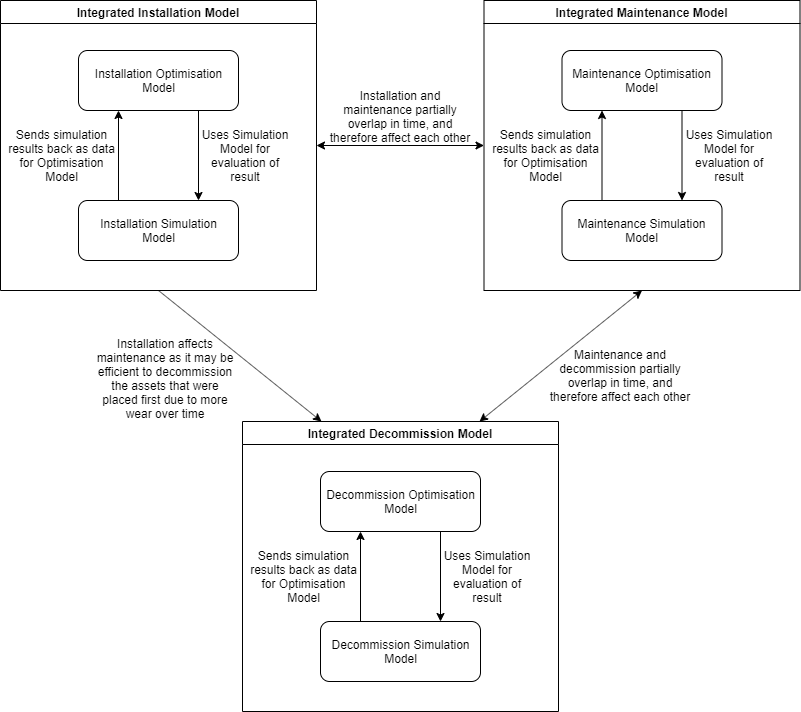
\includegraphics[width = \textwidth]{OWF Tool interactions}
\caption{The connections between each of the minor models that together make up the final model}
\label{f:interact}
\end{figure}

Installation and maintenance partially overlap in time, and therefore have a significant impact on each other. The scheduling of routing and time at ports for installation and maintenance vessels may benefit from being done together, and only the assets that have been installed require maintenance. Maintenance and decommission affect each other in a very similar way, as they too overlap in time. The direct influence is that near the end of the life-cycle, it may not be cost-efficient to maintain or repair an asset if it is to be decommissioned shortly after. Finally, installation affects decommission in more intricate ways. These phases do not overlap in time, but since the installation phase can take several years, some WTGs may be years older than other WTGs. This can affect maintenance, but also decommission as it may be cost-efficient to decommission the WTGs that are oldest first. However, there is more that affects this, as the maintenance on each individual asset can also influence the most cost-effective order of decommissioning. 

\bigskip

In practice there are various ways to integrate these models, and which works best will need to be explored and experimented with. In the decision support tool the simulation models should be simple to combine, effectively allowing for one big simulation. It would start simulating the installation project, and start the maintenance simulation once it reaches a certain milestone (probably the first turbines being finished). Installation would then finish up, and maintenance would continue until a certain point in time where decommission starts. How the optimisation model ties into this is not completely decided yet, and preferably the tool would have multiple options depending on the users preferences. For example a user might only want to optimise the installation schedule, but with regards to minimising life-cycle costs. Only the installation optimisation model would come into play, but all three simulation models are needed. In the tool, this is pretty straightforward, but in the theoretical models this may be more difficult to reflect. 

When multiple phases need to be optimised, this could theoretically be done by directly combining the models and having one big model with decision variables and constraints related to various phases. This will likely be a very large and computationally heavy model. A more practically feasible method will likely be a back-and-forth approach where one phase is optimised, and the corresponding decision variables are used in another phase as fixed values. This can be done back-and-forth for a set number of times or until no further optimisations are found. This is similar to combining the models and having a large number of decision variables, and using column generation to split the decision variables considered into manageable sets. 

In summary, the exact way this will be done is still under consideration, but there are some clear candidate approaches. 

\subsection{Timeline and next steps} \label{ss:timel}
%Timeline and focus from here
Since research is inherently exploratory and unpredictable, it is impossible to have a timeline set in stone. However, in this section I will sketch a possible timeline and outline what I will focus on from here, based on the previously mentioned directions. Note that this timeline is subject to change, especially the further into the future it predicts. 

\bigskip

My immediate focus will now go to filling in my knowledge gaps regarding the maintenance projects. As stated before, some research has already been conducted, but there is significant reading of the literature to be done, which I aim to do in the upcoming months. I am planning to do the bulk of this reading in the next two months, although more reading of the literature will naturally be something I do throughout this project. After the majority of this reading is done, I plan to work on the optimisation and simulation models for installation projects, and integrate them. I will then implement them into the tool described in \Cref{s:sim}, and getting it operational for installation projects while remaining adaptable enough to later be used in maintenance and decommission projects as well. The tool should be operational for that within the next six months. During this time, I will also attempt to contact industry partners to acquire real(istic) data. My supervisors have both worked extensively within this field so I am hopeful they will be able to help me connect to outside companies.

In the six months after that, I will attempt to design the models for both maintenance and decommission projects, in a similar structure to the model made for installation projects in order to improve compatibility. If data has been acquired from industry partners, some initial experiments to validate the tool up to this point will also be performed. After the models for each individual phase are completed, I will attempt to integrate them into one life-cycle spanning model. 

Hopefully all of that is completed 12-14 months from now. After that, the tool needs to be adapted for the full life-cycle model. Once that is completed, full validation of the tool can be done with the aquired data, and if successful some experimental analysis can be done. The extend on this heavily depends on the amount of time available. There are many directions to go in and possible improvements to add to the tool, but some of them will likely have to be carried out in some future research project. For example, the tool might benefit from realistic imperfect weather forecasts, which are uncommon in the current literature but potentially a way to improve accuracy. Additional optimisation methods can also be implemented, so that various methods can be compared and possibly combined. Experiments with location and layout of sites could also be added in the future, whether that is this PhD project or another future project. 

Finally a lot of writing on my PhD thesis will have to be done. I aim to write continuously throughout the project as it develops, using this report as a basis. However, at the end of the three years some time needs to be dedicated to finish up the writing. Ideally I will be able to complete this before the 3-year mark, but potentially the writing needs to be finished up in the few months afterwards. 

\bigskip

To summarise, this timeline would look like:

\begin{itemize}
	\item Year 2, second half: Read up more on maintenance projects and related research, design models for installation, implement those models in the tool, start initial contacts to acquire data
	\item Year 3, first half: Design models for maintenance and decommission projects, run initial simple experiments if data is available, start design on the life-cycle spanning integrated model
	\item Year 3, second half: Finish up the design of the model and implement it fully in the tool, validate tool and run analytical experiments. Writing will be kept up to data throughout the project, but it will be finalized at this time. 
\end{itemize}

In this scenario I am able to research the entire life-cycle of an OWF and build a tool for decision support at any point in that life-cycle. But as I stated before, this is a rough timeline, and is subject to change depending on where progress is made. If very promising initial results come from the installation part of the project, there is a chance the main focus will shift there, and maintenance projects fall to a background role. Naturally the opposite might also happen, or those good results may be found for the decommission projects. 

Writing additional papers is not included in this timeline, as this strongly depends on where significant results are found. However I would ideally publish at least one paper on the installation model, one on the maintenance model, and one on their combination. Writing them will have a strong overlap with writing the related chapters of my thesis, so this will coincide with the continual writing I am planning to do. 

\pagebreak

\bibliographystyle{agsm}
\bibliography{mybib}

%TODO: Uniformilize usage of I and We
%TODO: Go through all \Cref tags and check whether all claims made are correct

\end{document}